% Preambel
\documentclass[a4paper,openany]{report}


%\usepackage{a4wide}
\usepackage[ansinew]{inputenc}
\usepackage[T1]{fontenc}
\RequirePackage{ifpdf}

\usepackage{hyperref}
	\hypersetup{%
  colorlinks=true,   % activates colored references
  pdfpagemode=None,  % PDF-Viewer starts without content et.al.
  pdfstartview=FitH, % PDF-Viewer uses a defined page width
  %linkbordercolor=111,
  % citebordercolor=111,
  citecolor=blue,
  linkcolor=blue}

\ifpdf
  \usepackage[pdftex]{graphicx}
	  \DeclareGraphicsExtensions{.pdf}
\else
  \usepackage[dvips]{graphicx}
	  \DeclareGraphicsExtensions{.eps}
\fi

%\usepackage{asymptote}	
\usepackage{fancyhdr}
%\usepackage{supertabular}
\usepackage{booktabs}
%\usepackage{longtable}
%\usepackage[dvips]{rotating}
\usepackage{multirow}
\usepackage{multicol}

\usepackage{color}
\usepackage{amsmath}
\usepackage{alltt}
%\usepackage{array}
%\usepackage{colortbl}

%%%%%%%%%%%%%%%% will be used to defined a color scheme for
%%%%%%%%%%%%%%%% latex pages converted with "Highlight"
\newcommand{\hlstd}[1]{\textcolor[rgb]{0,0,0}{#1}}
\newcommand{\hlnum}[1]{\textcolor[rgb]{0.75,0,0.35}{#1}}
\newcommand{\hlesc}[1]{\textcolor[rgb]{0.42,0.35,0.8}{#1}}
\newcommand{\hlstr}[1]{\textcolor[rgb]{0.75,0,0.35}{#1}}
\newcommand{\hldstr}[1]{\textcolor[rgb]{0.75,0,0.35}{#1}}
\newcommand{\hlslc}[1]{\textcolor[rgb]{0.25,0.38,0.56}{#1}}
\newcommand{\hlcom}[1]{\textcolor[rgb]{0.25,0.38,0.56}{#1}}
\newcommand{\hldir}[1]{\textcolor[rgb]{0.8,0,0.8}{#1}}
\newcommand{\hlsym}[1]{\textcolor[rgb]{0,0,0}{#1}}
\newcommand{\hlline}[1]{\textcolor[rgb]{0.25,0.38,0.56}{#1}}
\newcommand{\hlkwa}[1]{\textcolor[rgb]{0.65,0.16,0.16}{\bf{#1}}}
\newcommand{\hlkwb}[1]{\textcolor[rgb]{0.18,0.55,0.34}{\bf{#1}}}
\newcommand{\hlkwc}[1]{\textcolor[rgb]{0.15,0.37,0.93}{\bf{#1}}}
\newcommand{\hlkwd}[1]{\textcolor[rgb]{0.32,0.11,0.78}{#1}}
\definecolor{bgcolor}{rgb}{1,0.85,0.73}
\oddsidemargin -3mm
\textwidth 165,2truemm
\topmargin 0truept
\headheight 0truept
\headsep 0truept
\textheight 230truemm
%%%%%%%%%%%%%%%%%%%%%%%%%%%%%%%%%%%%%%%%%%%%%%%%%%%%%%%

\clubpenalty = 10000
\widowpenalty = 10000 \displaywidowpenalty = 10000

\definecolor{hellgrau}{gray}{0.95}
\definecolor{dunkelgrau}{gray}{0.55}

\definecolor{brown}{rgb}{0.75,0.004,0.3}


\renewcommand{\headrulewidth}{0pt} % no head rule
\renewcommand{\footrulewidth}{0pt} % no footer rule

%\nointend
%%%%%%%%%%%%%%%%%%%%%%%%%%%%%%
% start text here!!


\begin{document}
\pagenumbering{roman}
% start text here!!

\title{A neural network package for Octave\\
		User's Guide \\
				Version: 0.1.9.1}

\author{Michel D. Schmid}
\maketitle


\tableofcontents
\pagenumbering{arabic}

\chapter{Introduction}
This documentation isn't a well defined and structured docu for the neural network toolbox.
It's more a \textit{collection of my ideas and minds}.


\section{Installed system}
I'm developing and testing the actual version of the neural network toolbox on following 
program versions:

\begin{itemize}
  \item Octave 2.9.5
  \item octave-forge-2006.01.28
  \item OctPlot svn version
\end{itemize}

.. and on another system

\begin{itemize}
  \item Octave 2.9.12
  \item octave-forge packages ...
  \item OctPlot svn version
\end{itemize}


\section{Version numbers}

The first number describes the major release. Version number V1.0 will be the first toolbox release which should have the same functions like the Matlab R14 SP3 neural network Toolbox.\\

The second number defines the finished functions. So to start, only the MLPs will realised and so this will be the number V0.1.0.\\

The third number defines the status of the actual development and function. V0.1.0 means a first release with MLP. Actually it works only with Levenberg-Marquardt algorithm and Mean-Square-Error as performance function.
\section{Code convention}

The main function of this toolbox will be programed with help of the book in \cite{4}.
So the variables will have the same names like in the book with one exception: Variables, only with one letter, will have two letters, e.g. 
\begin{itemize}
	\item $X \rightarrow Xx$
	\item $Q \rightarrow Qq$
	\item $a \rightarrow aa$
\end{itemize}
and so on ...\\

This is only to make it possible to search for variable names.



\chapter{Neural Network Package for Octave}
This chapter describes all functions available in the neural network package of Octave.

Eventhough it will be as compatible as possible to the one of MATLAB(TM).

\section{Available Functions}
\subsection{min\_max}
Checks for minimal and maximal values of an input matrix for \textbf{newff}.\\

\subsubsection{Syntax:}

$pr = min\_max(mInputs)$\\

\subsubsection{Description:}
\textit{mInputs} must be a matrix with input training data sets. This means in the case, for a 9-2-1 MLP
(this means 9 input-, 2 hidden- and 1 output-neuron) with 100 input training data sets, the matrix must be
an 9x100 matrix. \textit{pr} will then be a 9x2 matrix with minimal values in the first column and maximal values in the second column. If a row holds 2 zeros, a warning will appear (no information in this row!).

\subsubsection{Important:}
The equival function in MATLAB(TM) is called \textit{minmax}. This is not possible because the functions \textit{min} and \textit{max} in Octave are programed in minmax.cc!
\subsection{min\_max}
Checks for minimal and maximal values of an input matrix for \textbf{newff}.\\

\subsubsection{Syntax:}

$pr = min\_max(mInputs)$\\

\subsubsection{Description:}
\textit{mInputs} must be a matrix with input training data sets. This means in the case, for a 9-2-1 MLP
(this means 9 input-, 2 hidden- and 1 output-neuron) with 100 input training data sets, the matrix must be
an 9x100 matrix. \textit{pr} will then be a 9x2 matrix with minimal values in the first column and maximal values in the second column. If a row holds 2 zeros, a warning will appear (no information in this row!).

\subsubsection{Important:}
The equival function in MATLAB(TM) is called \textit{minmax}. This is not possible because the functions \textit{min} and \textit{max} in Octave are programed in minmax.cc!
\subsection{min\_max}
Checks for minimal and maximal values of an input matrix for \textbf{newff}.\\

\subsubsection{Syntax:}

$pr = min\_max(mInputs)$\\

\subsubsection{Description:}
\textit{mInputs} must be a matrix with input training data sets. This means in the case, for a 9-2-1 MLP
(this means 9 input-, 2 hidden- and 1 output-neuron) with 100 input training data sets, the matrix must be
an 9x100 matrix. \textit{pr} will then be a 9x2 matrix with minimal values in the first column and maximal values in the second column. If a row holds 2 zeros, a warning will appear (no information in this row!).

\subsubsection{Important:}
The equival function in MATLAB(TM) is called \textit{minmax}. This is not possible because the functions \textit{min} and \textit{max} in Octave are programed in minmax.cc!
\subsection{poststd}
\subsection{saveMLPStruct}
This is an additional function which doesn't exist in the neural network toolbox of MathWorks (TM). To see the network structure, you can use this command and save the complete structure to a file. Open this file and you have the same view like you would open the \textit{network type} of MATLAB(TM).\\

\noindent \textbf{\textcolor{brown}{Syntax:}}\\

\noindent saveMLPStruct(net,"initNetwork.txt");\\





\subsection{min\_max}
Checks for minimal and maximal values of an input matrix for \textbf{newff}.\\

\subsubsection{Syntax:}

$pr = min\_max(mInputs)$\\

\subsubsection{Description:}
\textit{mInputs} must be a matrix with input training data sets. This means in the case, for a 9-2-1 MLP
(this means 9 input-, 2 hidden- and 1 output-neuron) with 100 input training data sets, the matrix must be
an 9x100 matrix. \textit{pr} will then be a 9x2 matrix with minimal values in the first column and maximal values in the second column. If a row holds 2 zeros, a warning will appear (no information in this row!).

\subsubsection{Important:}
The equival function in MATLAB(TM) is called \textit{minmax}. This is not possible because the functions \textit{min} and \textit{max} in Octave are programed in minmax.cc!
\begin{verbatim}
%!shared matrix, nTargets, mTrain, mTest, mVali
%! disp("testing subset")
%! matrix = [1 2 3 4 5 6 7 8 9 10 11 12 13 14 15 16 17 18 18 20; \
%!			 0 2 4 1 3 5 3 4 1 -1 -2 -9 -1 10 12 20 11 11 11 11; \
%!			-2 2 2 2 2 0 0 0 0  0 10 12 13 12 13 44 33 32 98 11; \
%!			 0 0 0 0 1 1 1 1 0  0  1  1  1  0  0  1  1  1  0  0; \
%!           4 4 4 4 4 4 4 4 4  4  4  4  4  4  4  4  4  4  4  4; \
%!           1 2 3 4 5 6 7 8 9 10 11 12 13 33 44 55 66 77 88 99];
%! nTargets = 1; # the last row is equivalent to the target values.
%! [mTrain, mTest, mVali] = subset(matrix,nTargets);  ############################
%!assert(size(mTrain,2)==10);# 50% of 20
%!assert(size(mTest,2)==6);# 1/3 of 20 = 6 (floor)
%!assert(size(mVali,2)==4);# 1/6 of 20 = 4 (floor)
%! # It's not possible to test the column order with this call!
%! # randomizing is used! But all max and min values should be
%! # in the training set
%!assert(max(mTrain(1,:))==max(matrix(1,:)));
%!assert(min(mTrain(1,:))==min(matrix(1,:)));
%!assert(max(mTrain(2,:))==max(matrix(2,:)));
%!assert(min(mTrain(2,:))==min(matrix(2,:)));
%!assert(max(mTrain(3,:))==max(matrix(3,:)));
%!assert(min(mTrain(3,:))==min(matrix(3,:)));
%!assert(max(mTrain(4,:))==max(matrix(4,:)));
%!assert(min(mTrain(4,:))==min(matrix(4,:)));
%!
%!
%! [mTrain, mTest, mVali] = subset(matrix,nTargets,0);  ############################
%!assert(size(mTrain,2)==10);# 50% of 20
%!assert(size(mTest,2)==6);# 1/3 of 20 = 6 (floor)
%!assert(size(mVali,2)==4);# 1/6 of 20 = 4 (floor)
%!assert(mTrain==matrix(:,1:10));
%!assert(mTest==matrix(:,11:16));
%!assert(mVali==matrix(:,17:20));
%!
%!
%! [mTrain, mTest, mVali] = subset(matrix,nTargets,2);  ############################
%!assert(size(mTrain,2)==10);# 50% of 20
%!assert(size(mTest,2)==6);# 1/3 of 20 = 6 (floor)
%!assert(size(mVali,2)==4);# 1/6 of 20 = 4 (floor)
%!assert(max(mTrain(1,:))==max(matrix(1,:)));
%!assert(min(mTrain(1,:))==min(matrix(1,:)));
%!assert(max(mTrain(2,:))==max(matrix(2,:)));
%!assert(min(mTrain(2,:))==min(matrix(2,:)));
%!assert(max(mTrain(3,:))==max(matrix(3,:)));
%!assert(min(mTrain(3,:))==min(matrix(3,:)));
%!assert(max(mTrain(4,:))==max(matrix(4,:)));
%!assert(min(mTrain(4,:))==min(matrix(4,:)));
%!
%!
%! ## next test ... optimize twice
%! matrix = [1 2 3 4 5 6 7 20 8 10 11 12 13 14 15 16 17 18 18 9; \
%!			 0 2 4 1 3 5 3 4 1 -1 -2 -9 -1 10 12 20 11 11 11 11; \
%!			-2 2 2 2 2 0 0 0 0  0 10 12 13 12 13 44 33 32 98 11; \
%!			 0 0 0 0 1 1 1 1 0  0  1  1  1  0  0  1  1  1  0  0; \
%!           4 4 4 4 4 4 4 4 4  4  4  4  4  4  4  4  4  4  4  4; \
%!           1 2 3 4 5 6 7 8 9 10 11 12 13 33 44 55 66 77 88 99];
%! [mTrain, mTest, mVali] = subset(matrix,nTargets,2);  ############################
%!assert(max(mTrain(1,:))==max(matrix(1,:)));
%!assert(min(mTrain(1,:))==min(matrix(1,:)));
%!assert(max(mTrain(2,:))==max(matrix(2,:)));
%!assert(min(mTrain(2,:))==min(matrix(2,:)));
%!assert(max(mTrain(3,:))==max(matrix(3,:)));
%!assert(min(mTrain(3,:))==min(matrix(3,:)));
%!assert(max(mTrain(4,:))==max(matrix(4,:)));
%!assert(min(mTrain(4,:))==min(matrix(4,:)));
\end{verbatim}

\subsection{min\_max}
Checks for minimal and maximal values of an input matrix for \textbf{newff}.\\

\subsubsection{Syntax:}

$pr = min\_max(mInputs)$\\

\subsubsection{Description:}
\textit{mInputs} must be a matrix with input training data sets. This means in the case, for a 9-2-1 MLP
(this means 9 input-, 2 hidden- and 1 output-neuron) with 100 input training data sets, the matrix must be
an 9x100 matrix. \textit{pr} will then be a 9x2 matrix with minimal values in the first column and maximal values in the second column. If a row holds 2 zeros, a warning will appear (no information in this row!).

\subsubsection{Important:}
The equival function in MATLAB(TM) is called \textit{minmax}. This is not possible because the functions \textit{min} and \textit{max} in Octave are programed in minmax.cc!
\subsection{min\_max}
Checks for minimal and maximal values of an input matrix for \textbf{newff}.\\

\subsubsection{Syntax:}

$pr = min\_max(mInputs)$\\

\subsubsection{Description:}
\textit{mInputs} must be a matrix with input training data sets. This means in the case, for a 9-2-1 MLP
(this means 9 input-, 2 hidden- and 1 output-neuron) with 100 input training data sets, the matrix must be
an 9x100 matrix. \textit{pr} will then be a 9x2 matrix with minimal values in the first column and maximal values in the second column. If a row holds 2 zeros, a warning will appear (no information in this row!).

\subsubsection{Important:}
The equival function in MATLAB(TM) is called \textit{minmax}. This is not possible because the functions \textit{min} and \textit{max} in Octave are programed in minmax.cc!


\section{Transfer functions}
\subsection{logsig}

\begin{figure}[htb]
\centering
  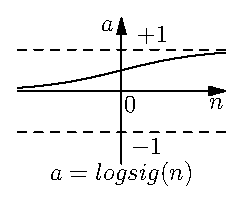
\includegraphics{octave/neuroPackage/graphics/logsig}
\caption{Log-Sigmoid transfer function}
\label{fig:logsigTransferFunction}
\end{figure}

\begin{figure}[htb]
\centering
  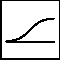
\includegraphics{octave/neuroPackage/graphics/logsiglogo}
\caption{Log-Sigmoid transfer function logo}
\label{fig:logsigTransferFunctionLogo}
\end{figure}
\subsection{purelin}

\begin{figure}[htb]
\centering
  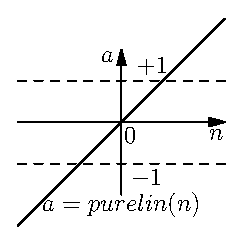
\includegraphics{octave/neuroPackage/graphics/purelin}
\caption{Linear transfer function}
\label{fig:purelinTransferFunction}
\end{figure}

\begin{figure}[htb]
\centering
  
\includegraphics{octave/neuroPackage/graphics/purelinlogo}
\caption{Linear transfer function logo}
\label{fig:purelinTransferFunctionLogo}
\end{figure}


\subsection{tansig}

\noindent
I solved all of my real life problems with this transfer function if a non-linear function was used. In [4] page 2-6 the tansig is defined as in equation \eqref{equ:tansigTransferFunction}. A look on the MathWorks homepage with the keyword tansig will show that tansig is programed as in equation \eqref{equ:tansigTransferFunctionNnet}.

\begin{equation}
	a = \frac{e^n - e^{-n}}{e^n + e^{-n}}
	\label{equ:tansigTransferFunction}
\end{equation}

\begin{equation}
	a = \frac{2}{(1 + e^{-2*n})-1}
	\label{equ:tansigTransferFunctionNnet}
\end{equation}


\begin{figure}[htb]
\centering
  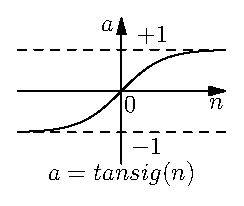
\includegraphics{octave/neuroPackage/graphics/tansig}
\caption{Tansig transfer function}
\label{fig:tansigTransferFunction}
\end{figure}

\begin{figure}[htb]
\centering
  
\includegraphics{octave/neuroPackage/graphics/tansiglogo}
\caption{Tansig transfer function logo}
\label{fig:tansigTransferFunctionLogo}
\end{figure}



\chapter{Examples}


\section{Example 1}

This MLP is designed with 2-2-1. This is not a complete example but it will help to understand the
dimensions of all matrices and vectores are used inside the Levenberg-Marquardt algorithm.

\subsection{Data matrices}
The input matrix will be defined like in equation \eqref{equ:mInput} and the output matrix like in 
equation \eqref{equ:mOutput}.

\begin{equation}
  mInput = \left[ \begin{array}{c c c c}
												1 & 2 & 3 & 1   \\
												1	& 1 & 1 & 2 	\\
												1 & 2 & 1 & 2		\\																					
												\end{array}
					\right]
		\label{equ:mInput}
\end{equation}

\begin{equation}
  mOutput = \left[ \begin{array}{c c c c}
												1 & 1.5 & 2 & 3   \\																					
									 \end{array}
					\right]
		\label{equ:mOutput}
\end{equation}




\subsection{Weight matrices}
The first layer matrix will hold 2x3 weights. The second layer matrix will hold 1x2 weights.
The first bias holds 3x1 weights and the second holds only a scalar element.

\subsection{Sensitivity Matrices}
This part is right now not so clear in my mind. What is the dimension of these two matrices?
The first layer sensitivity matrix should be about 2x71. Number of hidden neurons in the rows and number of train data sets in the columns.\\

In the actual version, the dimension is about 71x71 .. so it seems to have a mistake inside the algorithm :-(



% Preamble

%\documentclass[a4paper]{report}

%\usepackage[ngerman]{babel}
%\usepackage[T1]{fontenc}
%\usepackage[ansinew]{inputenc}


%%%%%%%%%%%%%%%%%%%%%%%%%%%%%%
% start text here!!

%\begin{document}

\begin{thebibliography}{XXXXXXX}

\bibitem [1]{1} John W. Eaton

GNU Octave Manual, Edition 3, PDF-Version, February 1997

\bibitem [2]{2} The MathWorks, Inc.

MATLAB Help, MATLAB Version 7.1 (R14SP3), Neural Network Toolbox Version 4.0.6 (R14SP3) 

\bibitem [3]{3} Christopher M. Bishop

Neural Networks for Pattern Recognition, OXFORD University Press, Great Clarendon Streed, Oxford OX2 6DP,
ISBN 0-19-853864-2, 2002

\bibitem [4]{4} Martin T. Hagen, Howard B. Demuth, Mark H. Beale

NEURAL NETWORK DESIGN, PWS Publishing Company, 20 Park Plaza, Boston, MA 02116-4324, ISBN 053494332-2, 1996

\end{thebibliography}
%\end{document}



\end{document}


